\chapter{Proposed Translator}
\label{ch:proposed-translator}

As a solution to the previous chapter, this one focuses on
proposing a application $f : S' \rightarrow M$ such that
applied on a schema, results in a domain model based on
plain objects.

Lets define $f(S') = \begin{bmatrix}f'(s_1')\\ f'(s_2')\\ \vdots\\ f'(s_n')\end{bmatrix}$ and
$f'(s_i') = \begin{bmatrix}f''(e_1')\\ f''(e_2')\\ \vdots\\ f''(e_n')\end{bmatrix}$. Then $f''(e_i')$
is the aplication that maps a triple expression $e'$ from $N \times T_{g} \times \{(1,1),(0,\infty)\}$
to $N \times T_g$. To find such a function we will use the knowledge that we already have.
We know that $p$ has a direct maping as it belongs to $N$, $T_g$ maps to $T_g$ if
the cardinality value is $(1,1)$ or $(1, \infty)$. And the cardinality is aggregated to the type
so its not needed to map it. Then we define the application $f''(e')$ as $f:(p,t,c) \in N \times T_g \times \{(1,1), (0,\infty)\} \rightarrow (n,t)\in N \times T_g$
and therefore,

\begin{equation}
f''(e_i')
\begin{cases}
    (p,Proy_{t_g}lst) & if \; c=(1,1) \\
    (p,List[Proy_{t_g}lst]) & if \; c=(0,\infty)
\end{cases}.
\end{equation}

This application's function is to transform a triple expression
into an annotated type property. Where the $Proy_{tg}lst$ represents
the projection of the generic type from the abstraction of languages
of representation of plain objects on to the language specific type.
\cref{fig:lst-diagram} illustrates how the same input can lead to
multiple types due to the specific translators, that perform the 
$Proy_{tg}lst$ operation.

\begin{figure}
    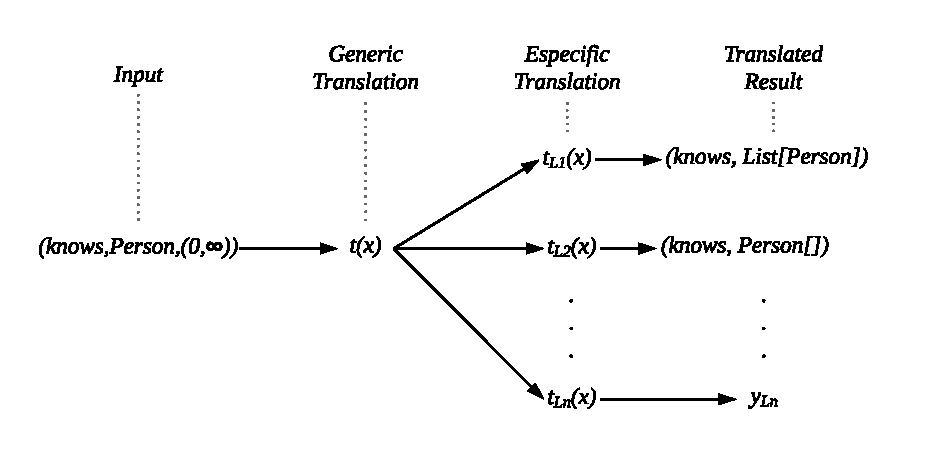
\includegraphics[scale=0.8]{images/lsc-diagram.pdf}
    \centering
	\caption[Diferent target types generated by specific translators]{Diferent target types generated by specific translators.}
    \label{fig:lst-diagram}
\end{figure}